\section{Camera calibration}

Camera calibration consists of estimating both intrinsic and extrinsic parameters to accurately model the imaging process.

\paragraph*{Intrinsic calibration}
The intrinsic calibration determines the camera's internal characteristics, specifically the calibration matrix $\mathbf{K}$ , which includes focal lengths, the principal point, and, in some cases, the skew factor $s$ (used in older cameras to account for non-square pixels or timing differences in sampling):
\[\mathbf{K}=\begin{bmatrix} f_x & s & U_0 \\ s & f_y & V_0 \\ 0 & 0 & 1 \end{bmatrix}\]

\paragraph*{Extrinsic calibration}
The extrinsic calibration estimates the camera's pose relative to the world coordinate system. 
This includes: 
\begin{itemize}
    \item The rotation matrix $\mathbf{R}$, which describes the camera's orientation.
    \item The translation vector $\mathbf{t}$, which defines the camera's position.
\end{itemize}
Unlike intrinsic parameters, extrinsic parameters change as the camera moves, affecting the transformation between world and image coordinates.

\subsection{Properties}
\paragraph*{Vanishing point}
A vanishing point $\mathbf{v}$ represents the image of a point at infinity along a given direction $\mathbf{d}$: 
\[\mathbf{U}_\mathbf{v}=\mathbf{Md}\]
Since the back-projection of the image point $\mathbf{v}$ is given by:
\[\mathbf{M}^{-1}\mathbf{u}_\mathbf{v}=\mathbf{MM}^{-1}\mathbf{d}=\mathbf{d}\] 
We can state the following theorem. 
\begin{theorem}
    The viewing ray associated with the vanishing point $\mathbf{v}$ of a direction $\mathbf{d}$ is parallel to $\mathbf{d}$.
\end{theorem}

\paragraph*{Viewing rays angle}
Given two image points $\mathbf{u}_1$ and $\mathbf{u}_2$, the angle $\theta$ between the directions of the lines connecting the camera center $\mathbf{C}$ to these points can be computed using the calibration matrix $\mathbf{K}$:
\[\cos\theta=\dfrac{\mathbf{u}_1^T\left(\mathbf{K}^{-T}\mathbf{K}^{-1}\right)\mathbf{u}_2}{\sqrt{\left(\mathbf{u}_1^T\left(\mathbf{K}^{-T}\mathbf{K}^{-1}\right)\mathbf{u}_1\right)\left(\mathbf{u}_2^T\left(\mathbf{K}^{-T}\mathbf{K}^{-1}\right)\mathbf{u}_2\right)}}\]
Since these angles are computed using only the intrinsic parameters, they are invariant to the absolute position of the camera.
By defining the image of the absolute conic as:
\[\boldsymbol{\omega}=\left(\mathbf{KK}^T\right)^{-1}\]
We obtain the following property.
\begin{property}
    The directions $\mathbf{d}_1$ and $\mathbf{d}_2$ of the viewing rays corresponding to two image points $\mathbf{u}_1$ and $\mathbf{u}_1$ form an angle given by: 
    \[\cos\theta=\dfrac{\mathbf{u}_1^T\boldsymbol{\omega}\mathbf{u}_2}{\sqrt{\left(\mathbf{u}_1^T\boldsymbol{\omega}\mathbf{u}_1\right)\left(\mathbf{u}_2^T\boldsymbol{\omega}\mathbf{u}_2\right)}}\]
\end{property}

\paragraph*{Circular points in space}
Each plane $\boldsymbol{\pi}$ has an associated pair of circular points, denoted as $\mathbf{I}_\mathbf{\pi}$, $\mathbf{J}_\mathbf{\pi}$. 
Notably, parallel planes share the same circular points.

To transform a reference $XY$ plane into a generic plane $\boldsymbol{\pi}$, we apply an isometric transformation $\mathbf{T}_{\boldsymbol{\pi}}$: 
\[\mathbf{T}_{\boldsymbol{\pi}}=\begin{bmatrix} & \mathbf{R}_{\boldsymbol{\pi}\mathbf{w}} & & \mathbf{o}_{\boldsymbol{\pi}} \\ 0 & 0 & 0 & 1 \end{bmatrix}\]
Which results in the following mappings for the circular points:
\[\mathbf{I}_{\boldsymbol{\pi}}=\mathbf{T}_{\boldsymbol{\pi}}\mathbf{I}_{XY}=\begin{bmatrix}\mathbf{R}_{\boldsymbol{\pi}\mathbf{w}}\mathbf{I} \\ \mathbf{0}\end{bmatrix} \qquad \mathbf{J}_{\boldsymbol{\pi}}=\mathbf{T}_{\boldsymbol{\pi}}\mathbf{J}_{XY}=\begin{bmatrix}\mathbf{R}_{\boldsymbol{\pi}\mathbf{w}}\mathbf{J} \\ \mathbf{0}\end{bmatrix}\]

\paragraph*{Plane and image homography}
Consider the homography $\mathbf{H}$ mapping points from a plane $\boldsymbol{\pi}$ to their corresponding image points.
\begin{figure}[H]
    \centering
    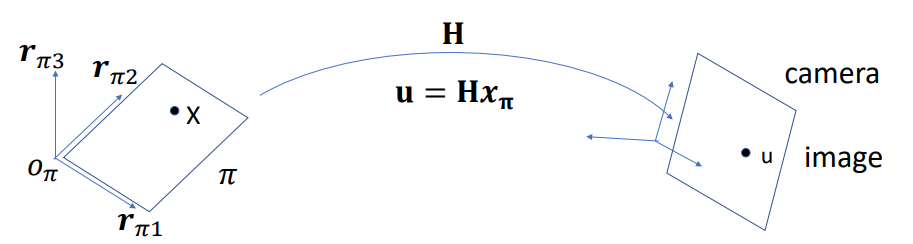
\includegraphics[width=0.75\linewidth]{images/plh.png}
    \caption{Plane homography}
\end{figure}
The plane $\boldsymbol{\pi}$ serves as a reference for determining its relative pose with respect to the camera, characterized by a rotation $\mathbf{R}_{\boldsymbol{\pi}}$ and translation $\mathbf{t}_{\boldsymbol{\pi}}$. 
The camera reference frame is taken as the world reference frame, with the projection matrix:
\[\mathbf{P}=\begin{bmatrix} \mathbf{K} & \mathbf{0} \end{bmatrix}\]
For a point $\mathbf{X}_{\boldsymbol{\pi}}$ on the plane, the homography is given by:
\[\mathbf{H}=\mathbf{K}\begin{bmatrix} \mathbf{r}_{\boldsymbol{\pi}\mathbf{1}} & \mathbf{r}_{\boldsymbol{\pi}\mathbf{2}} & \mathbf{o}_{\boldsymbol{\pi}} \end{bmatrix}\]
\begin{property}
    For any plane $\boldsymbol{\pi}$, the images of its circular points satisfy: 
    \[\mathbf{I}^\prime_{\boldsymbol{\pi}}\boldsymbol{\omega}\mathbf{I}_{\boldsymbol{\pi}}=\mathbf{0}\qquad\mathbf{J}^\prime_{\boldsymbol{\pi}}\boldsymbol{\omega}\mathbf{J}_{\boldsymbol{\pi}}=\mathbf{0}\]
\end{property}

\subsection{Calibration constraints}
To determine the calibration matrix $\mathbf{K}$, we can estimate the image of the absolute conic $\boldsymbol{\omega}$ and apply Cholesky factorization to its inverse.

The constraints on $\boldsymbol{\omega}$ can be derived from various geometric properties, including:
\begin{itemize}
    \item Known angles between directions, by analyzing their vanishing points.
    \item Self-orthogonality, by observing the images of circular points.
    \item Known planar shapes, by analyzing their image projections.
\end{itemize}
The main constraints that can be used to estimate $\boldsymbol{\omega}$ are: 
\begin{itemize}
    \item Known angles between directions $\mathbf{d}_i$ and their vanishing points. 
        If the directions $\mathbf{d}_i$ and their corresponding vanishing points $\mathbf{v}_i$ are known, where:
        \[\mathbf{v}_i=\mathbf{KRd}_i\]
        Then, the angle constraint between two directions is given by:
        \[\cos\theta=\dfrac{\mathbf{v}_1^T\boldsymbol{\omega}\mathbf{v}_2}{\sqrt{\left(\mathbf{v}_1^T\boldsymbol{\omega}\mathbf{v}_1\right)\left(\mathbf{v}_2^T\boldsymbol{\omega}\mathbf{v}_2\right)}}\]
    \item Images of the circular points. 
        The images of the circular points provide two independent equations, one for the real part and one for the imaginary part:
        \[\mathbf{I}^\prime_{\boldsymbol{\pi}}\boldsymbol{\omega}\mathbf{I}^\prime_{\boldsymbol{\pi}}=\mathbf{0}\]
    \item Known planar shapes and the homography $\mathbf{H}$ between image and scene. 
        If a homography $\mathbf{H}$ between the image and the scene is known, then we obtain the following two constraints:
        \[\mathbf{h}_1\boldsymbol{\omega}\mathbf{h}_2=\mathbf{0} \qquad \mathbf{h}_1\boldsymbol{\omega}\mathbf{h}_1-\mathbf{h}_2\boldsymbol{\omega}\mathbf{h}_2=\mathbf{0}\]
\end{itemize}

\subsection{Zhang method}
When performing camera calibration using images of multiple known planar shapes, we can apply Zhang's method to estimate the intrinsic matrix $\mathbf{K}$.
For each homography: $\mathbf{H}=\begin{bmatrix} \mathbf{h}_1 & \mathbf{h}_2 & \mathbf{h}_3 \end{bmatrix}$ we impose the following constraints on the image of the absolute conic $\boldsymbol{\omega}$:
\[\begin{cases} \mathbf{h}_1\boldsymbol{\omega}\mathbf{h}_2=\mathbf{0} \\ \mathbf{h}_1\boldsymbol{\omega}\mathbf{h}_1-\mathbf{h}_2\boldsymbol{\omega}\mathbf{h}_2=\mathbf{0} \end{cases}\]
These equations are homogeneous in $\boldsymbol{\omega}$, meaning that at least three homographies are required to fully determine $\boldsymbol{\omega}$.
Once $\boldsymbol{\omega}$ is estimated, we apply Cholesky factorization to its inverse to obtain the intrinsic calibration matrix $\mathbf{K}$.

\subsection{Camera calibration with camera position}
When the camera center position $\mathbf{O}$ is known, we can perform extrinsic and intrinsic calibration using a single image of a known planar shape. 
The calibration process follows these steps:
\begin{enumerate}
    \item Compute the homography $\mathbf{H}$ between known points on the plane $\boldsymbol{\pi}$ and their corresponding image points.
    \item Define the transformation matrix $\mathbf{M}_{\mathbf{o}}$ that relates any point $\mathbf{x}$ on $\boldsymbol{\pi}$ to the direction $\mathbf{d}$ of a ray from the camera center $\mathbf{O}$:
        \[\mathbf{M}_{\mathbf{o}}^{-1}=\begin{bmatrix} 1 & 0 & -x_{\mathbf{o}} \\ 0 & 1 & -y_{\mathbf{o}} \\ 0 & 0 & -z_{\mathbf{o}} \end{bmatrix}\]
    \item Compute the projection matrix $\mathbf{M}$ relating any image point $\mathbf{u}$ to the direction $\mathbf{d}$ of its viewing ray: 
        \[\mathbf{d}=\mathbf{M}_{\mathbf{o}}^{-1}\mathbf{H}^{-1}\mathbf{u}=\mathbf{M}^{-1}\mathbf{u}\]
    \item Perform a QR decomposition on $\mathbf{M}^{-1}$. 
        The decomposition $\mathbf{M}^{-1}=\mathbf{R}^{-1}\mathbf{K}^{-1}$ allows us to extract: $\mathbf{K}$, the intrinsic calibration matrix, and $\mathbf{R}^{-1}$, the rotation matrix from the world reference (attached to $\boldsymbol{\pi}$) to the camera.
\end{enumerate}

\subsection{Camera calibration with unknown scene}
When the shape of the scene is unknown but we have some images of it, we can perform camera calibration using a method that is generally less precise than the Zhang method. 
The process is as follows:
\begin{enumerate}
    \item Capture images of the scene using a camera with a constant intrinsic matrix $\mathbf{K}$.
    \item Compute the homographies between different images of the scene.
    \item Formulate the system of equations:
        \[\begin{cases}\mathbf{I}^{\prime T}\boldsymbol{\omega}\mathbf{I}^{\prime}=\mathbf{0} \\ \mathbf{I}^{\prime T}\mathbf{H}^{\prime T}\boldsymbol{\omega}\mathbf{H}^{\prime}\mathbf{I}^{\prime}=\mathbf{0}\end{cases}\]
    \item Solve for $\boldsymbol{\omega}$ and $\mathbf{I}^{\prime}$. 
    \item Compute the inverse matrix $\boldsymbol{\omega}^{-1}$ and perform a Cholesky factorization to find $\mathbf{K}$.
\end{enumerate}

\subsection{Camera calibration with natural camera}
Calibration of natural cameras (where $f_X=f_Y=f$) can be performed using the vanishing points of mutually orthogonal directions.

In this case, the image of the absolute conic $\boldsymbol{\omega}$ matrix has the following form:
\[\boldsymbol{\omega}=\begin{bmatrix} 1 & 0 & -U_0 \\ \ast & 1 & -V_0 \\ \ast & \ast & f^2+U_0^2+V_0^2 \end{bmatrix}\]
This matrix can be determined by solving the following system of three equations involving the vanishing points $\mathbf{v}_1$, $\mathbf{v}_2$, and $\mathbf{v}_3$:
\[\begin{cases} \mathbf{v}_1^T\boldsymbol{\omega}\mathbf{v}_2=\mathbf{0} \\ \mathbf{v}_2^T\boldsymbol{\omega}\mathbf{v}_3=\mathbf{0} \\ \mathbf{v}_3^T\boldsymbol{\omega}\mathbf{v}_1=\mathbf{0} \end{cases}\]

\subsection{Calibration from reconstructed shape and normal vanishing point}
In this calibration method, we use a planar face with a known (reconstructed) shape and a vanishing point of the normal to the plane.
The image of the absolute conic matrix $\boldsymbol{\omega}$ in this case is:
\[\boldsymbol{\omega}=\begin{bmatrix} a^{2} & 0 & -u_0a^{2} \\ \ast & 1 & -v_0 \\ \ast & \ast & f^2_Y+a^2u_0^2+v_0^2 \end{bmatrix}\]
Here, $a$ represents the pixel aspect ratio. 
To fully define this matrix, we need four equations:
\[\begin{cases}
    \mathbf{h}_1^T\boldsymbol{\omega}\mathbf{h}_2=\mathbf{0} \\
    \mathbf{v}^T\boldsymbol{\omega}\mathbf{h}_4=\mathbf{0} \\
    \mathbf{v}^T\boldsymbol{\omega}\mathbf{h}_1=\mathbf{0} \\
    \mathbf{v}^T\boldsymbol{\omega}\mathbf{h}_2=\mathbf{0} \\
\end{cases}\]
These equations allow us to solve for $\boldsymbol{\omega}$. 
Once we have $\boldsymbol{\omega}$, we can use Cholesky factorization on its inverse to obtain the camera calibration matrix.

\paragraph*{Direct method}
The direct method is independent of the chosen pairs of mutually orthogonal vanishing points. 
It works from:
\begin{enumerate}
    \item The reconstructed homography $\mathbf{H}_R$ from the given image to the rectified image.
    \item The image of the line at infinity $\mathbf{l}^{\prime}_{\infty}$, or the vanishing point $\mathbf{v}$ along the direction orthogonal to the face.
\end{enumerate}
Consider the plane-to-image homography $\mathbf{H}=\begin{bmatrix} \mathbf{h}_1 & \mathbf{h}_2 & \mathbf{h}_3 \end{bmatrix}=\mathbf{H}_R^{-1}$.
Additionally, the line at infinity $\mathbf{l}^{\prime}_{\infty}=\mathbf{v}_1\times \mathbf{v}_2$.
From this, we can extract the following constraints:
\[\begin{cases}
    \mathbf{h}_1^T\boldsymbol{\omega}\mathbf{h}_2 = \mathbf{0} \\
    \mathbf{h}_1^T\boldsymbol{\omega}\mathbf{h}_1 - \mathbf{h}_2^T\boldsymbol{\omega}\mathbf{h}_2 = \mathbf{0} \\ 
    \mathbf{l}_{\infty}^{\prime}=\boldsymbol{\omega}\mathbf{v}
\end{cases}\]
The last term of the system gives two equations.

Alternatively, we can impose the following constraints:
\[\begin{cases}
    \mathbf{h}_1^T\boldsymbol{\omega}\mathbf{h}_2 = \mathbf{0} \\
    \mathbf{h}_1^T\boldsymbol{\omega}\mathbf{h}_1 - \mathbf{h}_2^T\boldsymbol{\omega}\mathbf{h}_2 = \mathbf{0} \\ 
    \mathbf{v}^T\boldsymbol{\omega}\mathbf{h}_1=\mathbf{0} \\ 
    \mathbf{v}^T\boldsymbol{\omega}\mathbf{h}_2=\mathbf{0}
\end{cases}\]